%This is chapter 1
%%=========================================
\chapter{Introduction}
Computer science world and research which involves computation-based experiments have complex processes and interactions of embedded and real-time systems, compilers, networking, and operating systems. Unfortunately, with growing system complexity, it is getting more difficult to get the same results and conclusions which are provided by original scientific work which is leading to decreasing quality of research. That is why research world came with Re* research concept. \emph{Re* research} refers to processes with outputs and documentation which ensure \emph{repeatable, reproducible, recomputable, reusable} or \emph{replicable} results. In the scientific community, there is increasing concern about these characteristics, as evidenced by recent reports from ACM, Dagstuhl, and other players. The goal of this work is to consolidate and structure the knowledge around Re* research as well as the reflection and reception in the scientific community, including in conference and journal and submission requirements. All these best practices will lead to general paper and research quality improving.

%%=========================================
\section{Motivation}
Publications are one of the most critical and essential foundations of academic life. At the same time Jan Vitek\cite{DBLP:conf/emsoft/VitekK11} tells that computational disciplines have much more advantages in comparison with other fields of science since in most cases conferences plays the role of a filter for selecting the best scientific works. Unfortunately, due to the short publication time and the one-stage process of reviewing papers, the conferences had a profound impact on how the procedures in research are now being carried out. To remain competitive due to time constraints and unregulated standards of reproducibility of scientific works, most researchers had to decrease the level of research quality and not spend the majority of time to prepare, provide and publish code and documentation. Also, due to the increasing complexity of scientific experiments with the rapid growth of technical progress, as well as the fact that the main criteria for most conferences in the evaluation of scientific papers are the level of novelty - most Re*research concepts are increasingly ignored during publication writing.\par
In our days for computational-based experiments, all the processes that are performed while writing scientific work can be characterized as follows: \par
The researcher identifies the problem that has not yet been solved or solved non-effectively. In the future, the software is written, which conducts evaluation and tests of the task/problem. When programming is complete,  initiated the process of preparation of the initial data that will be processed by the software. When the result data is ready, it is analyzed by researcher and proofs hypothesis or creates brand new ideas based on the data. This workflow is shown in the picture: \ref{fig:workflow} \par
\begin{figure}[h!]
  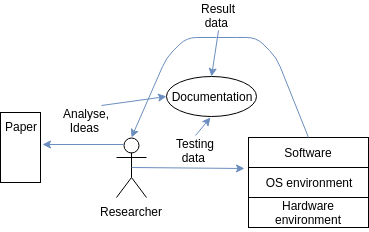
\includegraphics[scale=0.8]{fig/reresearch.png}
  \caption{Research workflow\cite{gith}}
  \label{fig:workflow}
\end{figure}

\par By Jan Vitek\cite{DBLP:conf/emsoft/VitekK11} the essence of the scientific process in computer systems consists of:
\begin{itemize}
    \item Identifying a problem and positing a hypothesis or model.
    \item Engineering a concrete implementation.
    \item Designing and conducting an experimental evaluation.
\end{itemize} \par

\section{Problem statement}
Experiments which includes computations, commonly represent complex ideas, and it is necessary to carry out a lot of tests on various of hardware and software platforms with several implementations. Typically, this is beyond the limitations caused by the amount of time and paper size. As a result, documents and scientific works that can be useful to the academic community are published without sufficient documentation, mention of restrictions and adequate instructions to reproduce the experiment and results. \par
Reasons above led to the fact that the academic community came to the idea of Re* research. Re* research refers to processes with outputs and documentation which ensure repeatable, reproducible, recomputable, reusable or replicable results. Instead, by Collberg\cite{DBLP:journals/cacm/CollbergP16} the symptoms of the current state of practice include:
\begin{itemize}
    \item Unrepeatable results
    \item Unreproduced results 
    \item Measuring the wrong thing 
    \item Meaninglessly measuring the right thing. 
\end{itemize} \par
Jan Vitek\cite{DBLP:conf/emsoft/VitekK11} defines more factors apart from pressure which are leading to bad quality from Re* research point of view:
\begin{itemize}
    \item Lack of benchmarks
    \item Lack of experimental methodology
    \item Lack of understanding of statistical methods
\end{itemize}
Tomas Kalibera in his work\cite{DBLP:conf/popl/Vitek15} "Repeatability, reproducibility in computer systems research" defines 7 "Deadly sins" in research which are making end results much useless :
\begin{itemize}
    \item \textbf{"Unclear experimental goals."} First of all, it is necessary to formulate the purpose of the experiment and what kind of results and conclusions are expected in the end. Without clearly posed questions, the experiment has not much sense.
    \item \textbf{"Implicit assumptions or experimental methodology."}. The documentation should have full information about the experimental setup and methodology that were used in conducting the experiment.
    \item \textbf{"Proprietary benchmarks and data sets."} For many researchers, as well as for industry, the availability of benchmarks and data sets used in the experiment could be a key point.
    \item \textbf{"Weak statistical analysis."} Even at high-level conferences like PLDI’11 \cite{DBLP:conf/pldi/2011}, most of the works ( 39 of 42) did not mention about the division in a time of executed experiments.
    \item \textbf{"Measuring the wrong thing/right thing meaninglessly."} Often a situation occurs when complex and non-trivial experiments involve incorrect connections between various factors.
    \item \textbf{"Lack of a proper baseline."} Many researchers while writing a paper use own implemented baseline with differing levels of optimization. Therefore, it is essential at the beginning of the experiment to establish a reliable and credible baseline.
    \item \textbf{"Unrepresentative workloads."} One of the biggest dangers of writing a regular paper is the wrong load on the computer system. Processes that performs in parallel with the conducted experiment can have a fundamentally affect on the result and could not be reproduced in the future.
\end{itemize}
\section{Methodology}
To write this survey paper, scientific papers, articles, and posts were analyzed. Most of the time, data sources were found and taken from both DBLP\cite{dblp} and Google Scholar\cite{google}. In total, 75 scientific papers were analyzed, and for each of the characteristics of the Re* research, 3-5 papers were selected. The analysis of the scientific material was carried out to compile a general picture and the relationship between the characteristics given above, each of which is central in a variety of scientific publications. All the selected scientific works were abstracted on the problem they cover, and year of publishing. The figure\ref{fig:figure1} shows a graph with the number of publications where certain characteristic was a central problem. For making this analysis, the full list of papers was used (see Appendix) and simple Python code which together with initial data can be found on GitHub\cite{gith}. 
\begin{figure}[h!]
\hspace*{-1.5cm}  
  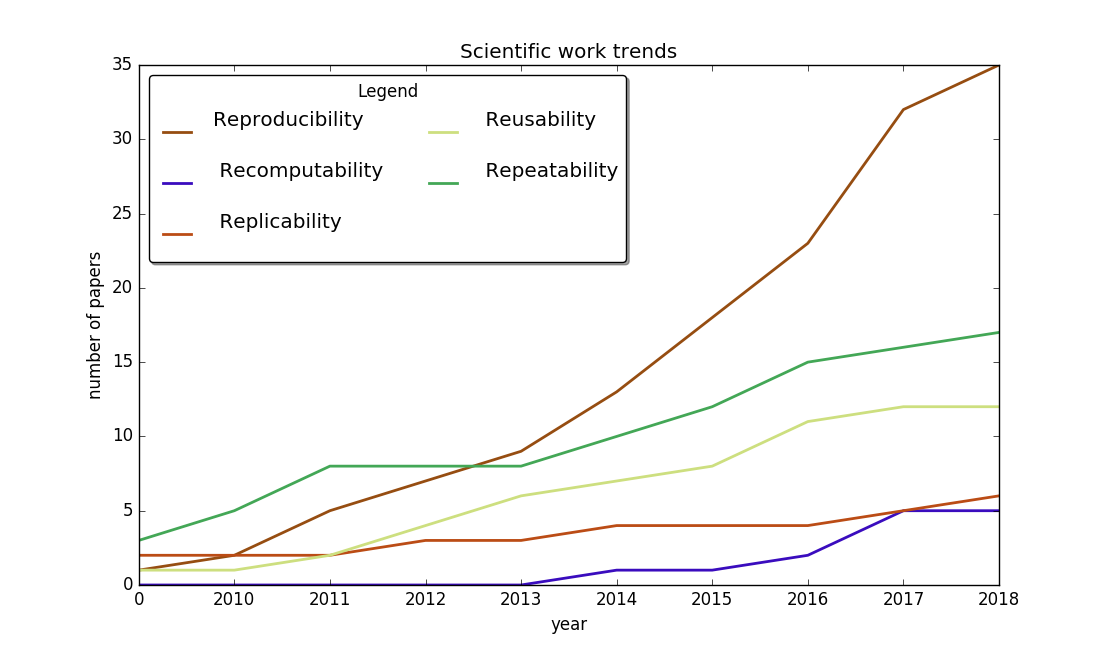
\includegraphics[scale=0.7]{fig/figure1.png}
  \caption{Paper analysis\cite{gith}}
  \label{fig:figure1}
\end{figure} \par
The primary requirements were the quality of the paper, documents with later dates had a privilege and, of course, papers were chosen which determined the research characteristics of Re *research as a central topic. From the analyzed articles, the most prominent efforts were made to extract definitions, features, current solutions and generalize them to give a clear idea of these topics separately and to create a "general view" of the study. The "general view" implied a clear division and commonalities between each part of the Re* study. As a result, the goal was also to make a set of simple requirements that will help make scientific work reproducible/repeatable/recomputable/reusable/replicable.